\subsection{Automatic text annotation}
We automatically annotated the documents using a \emph{Stanza} \cite{stanza} pipeline: this operation consisted of:
\begin{itemize}
    \item Tokenization
    \item Part of speech tagging
    \item Lemma extraction
    \item Dependency parsing
\end{itemize}

Before this step we preprocessed the text in order to remove mentions, urls and normalize the punctuation: in particular sequences of multiple full stops were reduced to one full stop, since they were creating issues with the sentence tokenization.
As for hashtags, since often single words hashtags are integrated in the syntax of the sentence we decided to remove only the hash symbol and preserve the textual part of the hashtags.

Our choice of using Stanza was predicated on the possibility of using a combined model based on several different treebanks for the Italian language.
This allowed us to get a better coverage of the language, which is particularly important when working on a non standard variety like tweets or in general computer mediated writing.
In particular, the combined model is based on four treebanks ISDT, VIT, PoSTWITA and TWITTIRO: the latter two were developed specifically for the annotation of tweets.

\subsection{Linguistic profiling}
With the objective of identifying, if possible, stylistic features useful for hate speech detection, we developed 91 different features for the linguistic profiling of the text belonging to five different categories:

\begin{itemize}
    \item{\textbf{Raw text properties:}} text length in terms of number of tokens and number of sentences. Average length of sentences and words as a really simple proxy of syntactic complexity;
    \item{\textbf{Social media language properties:}} distribution of URLs, hashtags, mentions and all uppercase words;
    \item{\textbf{Lexical variety}} expressed in terms of Type/Token Ratio;
    \item{\textbf{Morpho-syntactic properties}}, namely the distribution of all grammatical categories and lexical density (proportion of content words in the text);
    \item{\textbf{Syntactic properties:}} distribution of all dependency relationships and relative order of core arguments and verb in sentences. Another aspect that received some attention was the distribution of nominal sentences, since the literature suggested a strong association between Slogan-like nominal utterances and hateful content \cite{comandini_nominal_utterances}.
\end{itemize}

In order to get some insights in the challenges associated with the cross-domain task, we scraped headlines from the online editions of \emph{La Stampa}, \emph{La Repubblica}, \emph{Il Giornale} and \emph{Liberoquotidiano}.
We filtered the headlines for the presence of the same small set of neutral keywords associated with immigrants, muslims and Roma used for the creation of the original dataset of tweets \cite{poletto_hate_2017}.

We thus obtained 748 newspapers headlines, which we passed to the automatic text annotation pipeline and analyzed stylistically.
We then trained a Linear Support Vector Machine on the linguistic profiling features in order to determine which features contributed the most in distinguishing between tweets and headlines. The classifier was able to distinguish tweets from headlines with near certainty, obtaining a macro-F1 of 0.949 in 5-fold cross validation.

As expected, social media properties like the number of mentions, hashtags, URLs and the use of uppercase, were mainly responsible for the success of the classifier. In addition to that, the feature importance analysis seems to indicate that tweets tend to be longer and have longer sentences than headlines; on the other hand, headlines seem to use more punctuation and more proper nouns and exhibit higher lexical variety (but since the Type/Token Ratio measure is highly sensitive to text length, this is probably a spurious result).
Figure \ref{fig:style} shows the distributions of several linguistic profiling features (document length in tokens, average sentence length, distribution of punctuation, distribution of proper nouns and Type/Token Ratio by form) for tweets and headlines.
Although the distributions are overlapping, it is possible to discern clear trends that confirm the results of the feature importance analysis.

\begin{figure}
    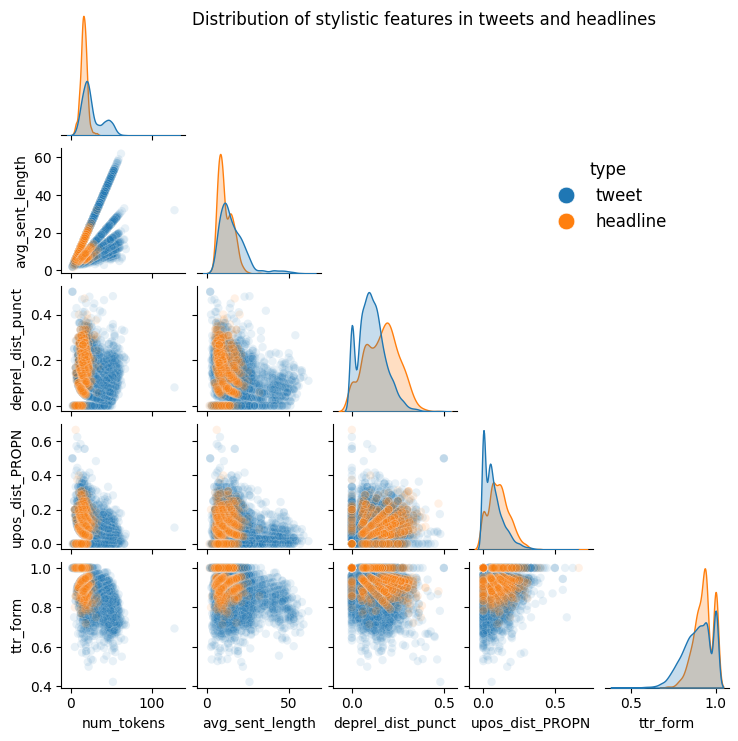
\includegraphics[width=\columnwidth]{../../results/images/style.png}
    \caption{Comparat{}ive stylistic analysis of tweets and scraped headlines.}
    \label{fig:style}
\end{figure}